\chapter{DEVOPS}
\label{chap:devops}

This chapter displays the project's Continuous Integration and Continuous Deployment set up that allows automated builds, tests, releases, and more. Having a correct setup is key to enhance productivity and let developers focus on coding instead of repetitive tasks like deploying.

% \vfill
% \begin{figure}[ht!]
%     \center
%     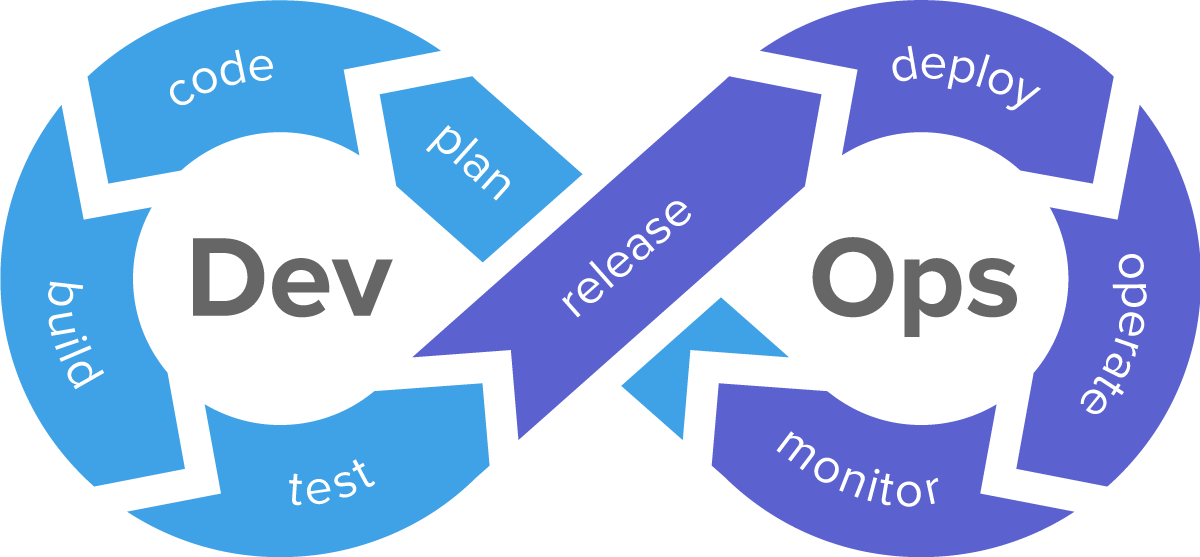
\includegraphics[width=0.75\textwidth]{media/devops.png}
%     \caption{Typical DevOps cycle}
%     \label{fig:devops}
% \end{figure}
% \vfill

% \clearpage\newpage
\section{Continuous integration}
\label{sec:ci}

Continuous integration (CI) is the practice of routinely integrating code changes into the main branch of a repository, and testing the changes, as early and often as possible. Ideally, developers will integrate their code daily, if not multiple times a day \cite{ci-definition}.

\vfill
\begin{figure}[ht!]
    \center
    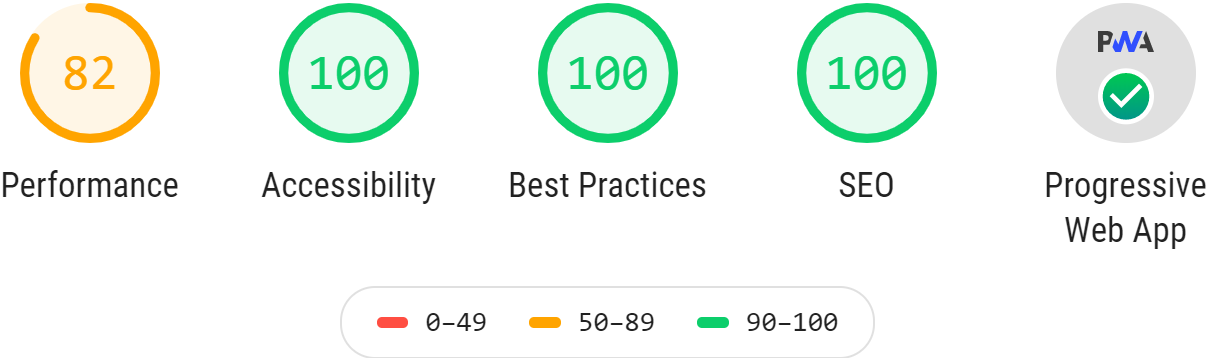
\includegraphics[width=0.9\textwidth]{media/lighthouse-score.png}
    \caption{Lighthouse score of GradeCalc}
    \label{lighthouse-score}
\end{figure}
\vfill

\clearpage\newpage\noindent

Every time a commit happens, the ci pipeline starts. In this project, three processes start in parallel:
\begin{enumerate}[itemsep=0mm]
    \item \textbf{Code Climate} runs a static code analysis and generates a score and a report with suggestions.
    \item \textbf{Netlify} builds the page and generates a deploy preview, more details in section \ref{sec:cd}.
    \item \textbf{Travis CI} builds the page and runs several processes:
    \begin{enumerate}[itemsep=0mm]
        \item \textbf{Automated test suite}: runs unitary tests.
        \item \textbf{Linterns}: checks that the code style follows a standard and is consistent. The lintern used is ESLint.
        \item \textbf{Lighthouse}: audits the page for performance, accessibility, progressive web apps, and SEO, and generates a report with detailed information about the issues and how to fix them.
    \end{enumerate}
\end{enumerate}

\vfill
\begin{figure}[ht!]
    \center
    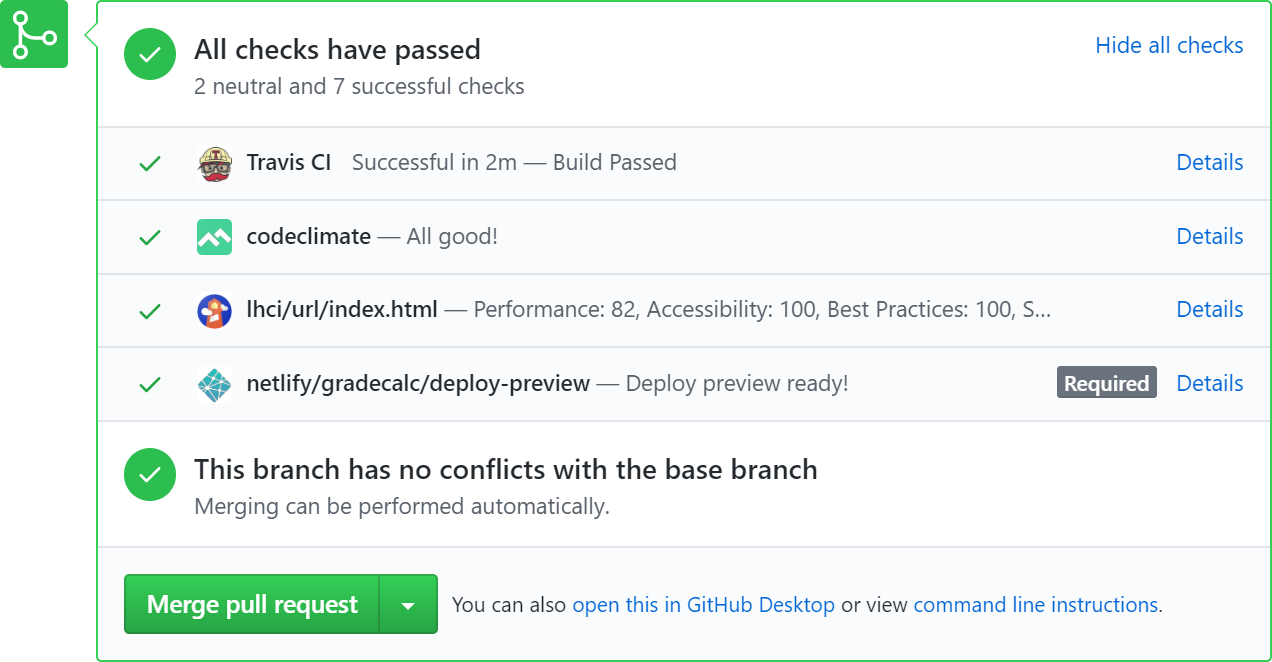
\includegraphics[width=\textwidth]{media/screenshot-pr.png}
    \caption{Pull request checks of GradeCalc}
    \label{pr}
\end{figure}
\vfill

\clearpage\newpage\noindent
Other processes are not triggered by commits, but for other events:
\begin{enumerate}[itemsep=0mm]
    \item \textbf{Dependabot} retrieves the dependency files, looks for any outdated or insecure dependency, and opens pull requests to update each requirement individually.
    \item \textbf{Stale} automatically close stale Issues and Pull Requests that tend to accumulate during the project.
    \item \textbf{Imgbot} watches for new images in the repository and opens pull requests optimizing those.
\end{enumerate}


% \vfill
% \begin{figure}[ht!]
%     \center
%     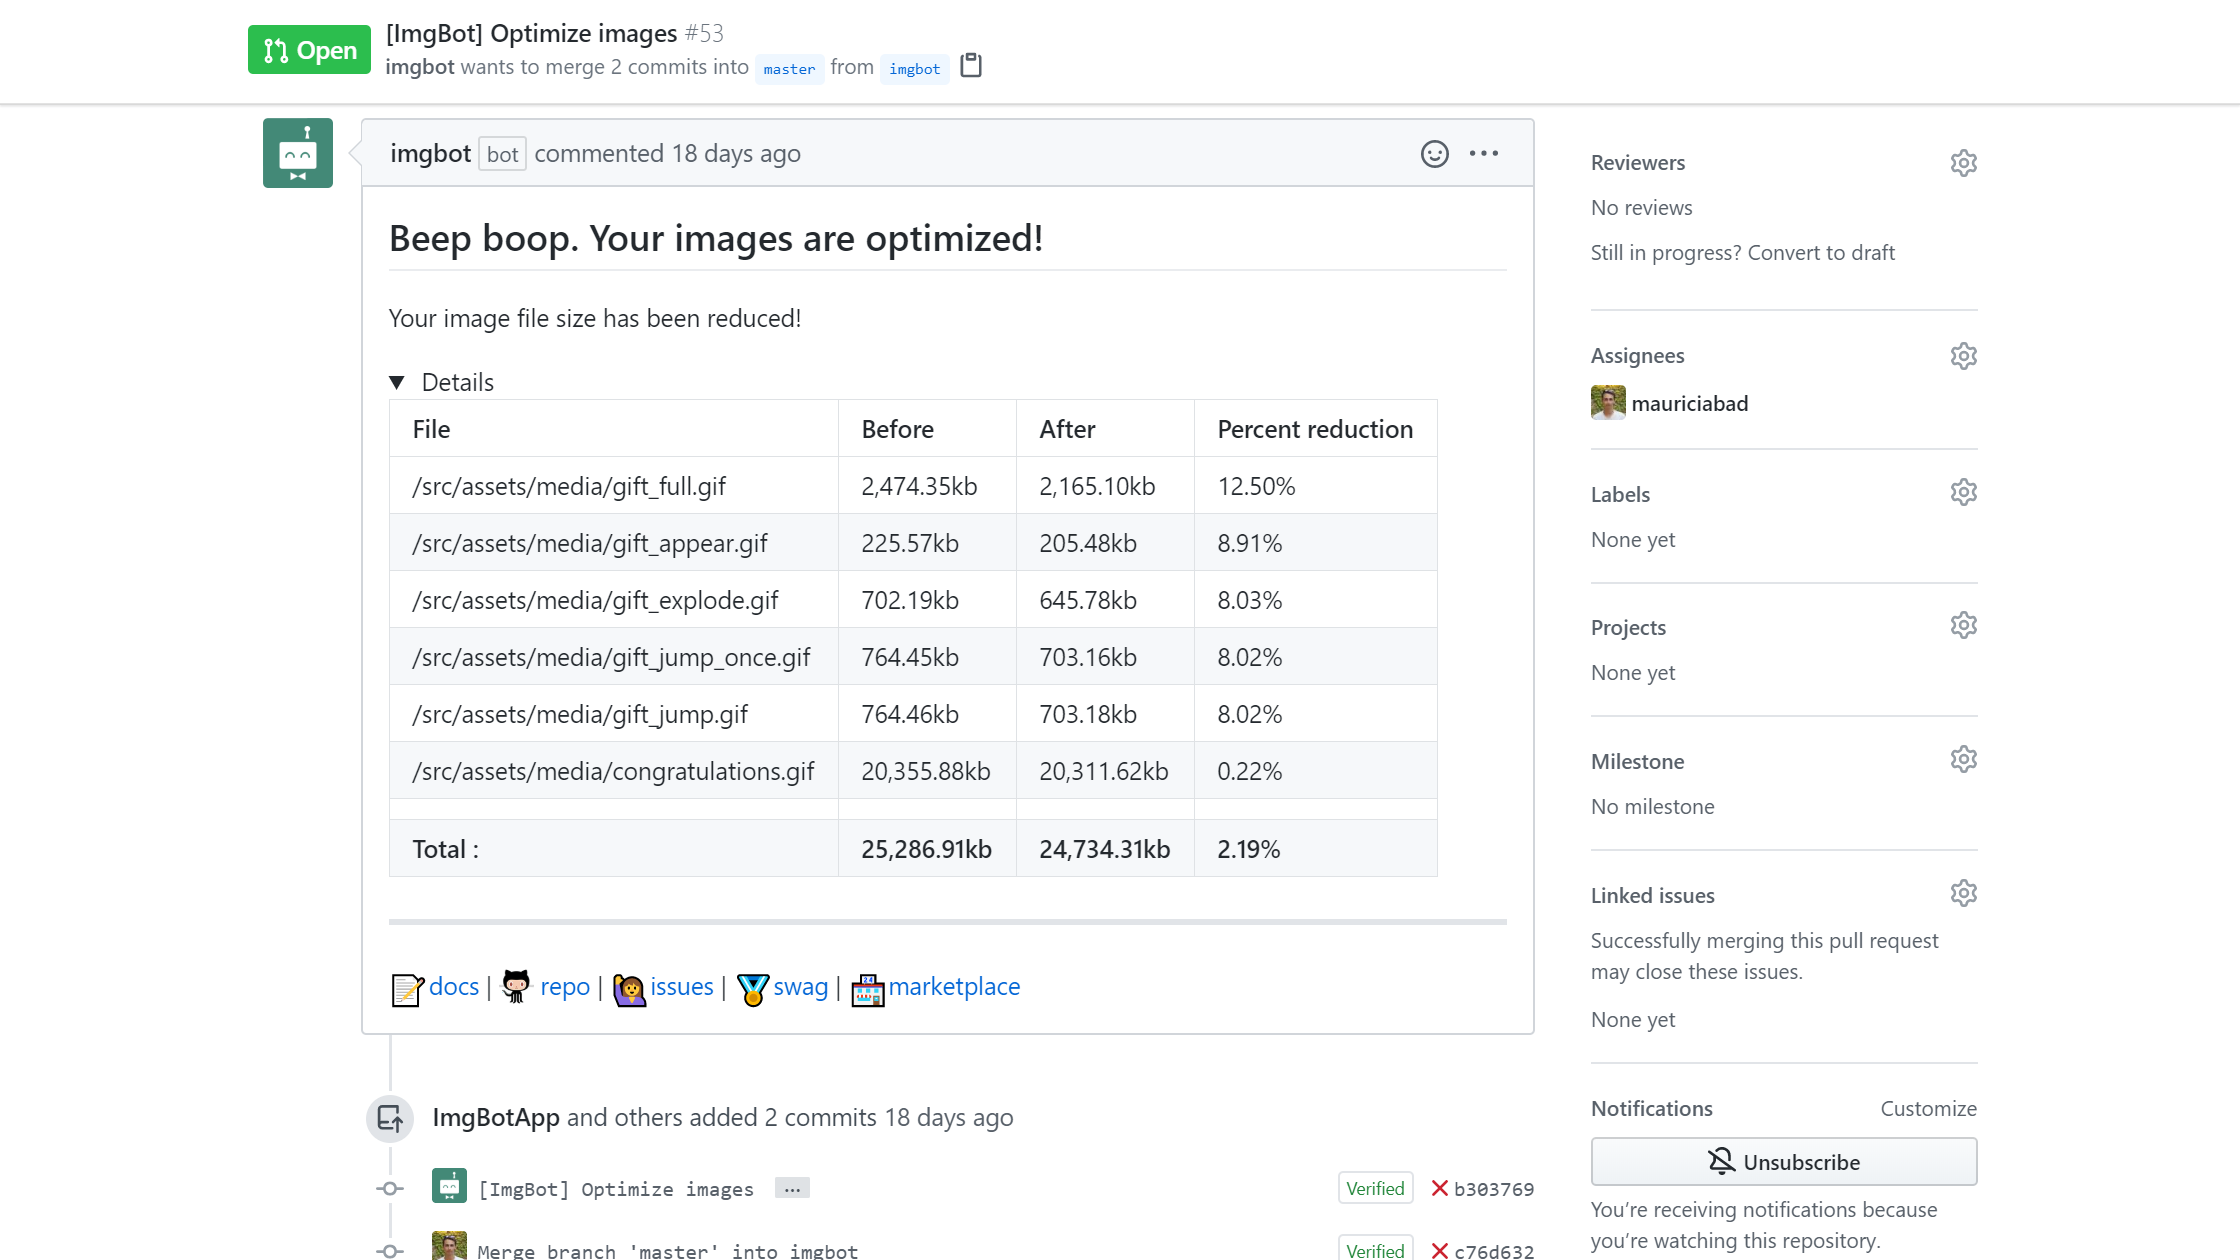
\includegraphics[frame,width=\textwidth]{media/screenshot-imgbot-pr.png}
%     \caption{Imgbot pull request in GradeCalc}
%     \label{imgbot-pr}
% \end{figure}

\clearpage\newpage\noindent
\section{Continuous deployment}
\label{sec:cd}

Continuous deployment (CD) is an approach in which software functionalities are delivered frequently through automated deployments. In contrast to occasionally releasing many changes at once. 

The benefits that CD provides are many, the ones that favor this project are:
\begin{itemize}[itemsep=0mm]
    \item Developers don't have to worry about deploys and they can focus on code. Deploys happen seamlessly without problems.
    \item Removes any human errors during the deployment process.
\end{itemize}

\noindent
This project's CD setup is entirely handled by Netlify, they describe themselves as follows:
\blockquote{Netlify is an all-in-one platform for automating modern web projects. Replace your hosting infrastructure, continuous integration, and deployment pipeline with a single workflow. Integrate dynamic functionality like serverless functions, user authentication, and form handling as your projects grow. \cite{netlify-docs}}
This is how Netlify is used in this project: 

In every commit, Netlify builds the page. In each build, a deploy preview is generated. This preview used for testing in a pre-production environment, and once everything works fine the changes can be merged into the master branch. 

Once a commit happens in master, either from a merge or a direct commit, Netlify builds the page, and if it builds successfully it is deployed into Netlify's powerful hosting infrastructure, in our case this is production. 

To build the page Netlify uses the npm command \mintinline{bash}{npm run dist}. That command creates a \texttt{dist/} folder that contains all the files that need to be hosted. These files are optimized versions of the source code.

% \vfill
% \begin{figure}[ht!]
%     \center
%     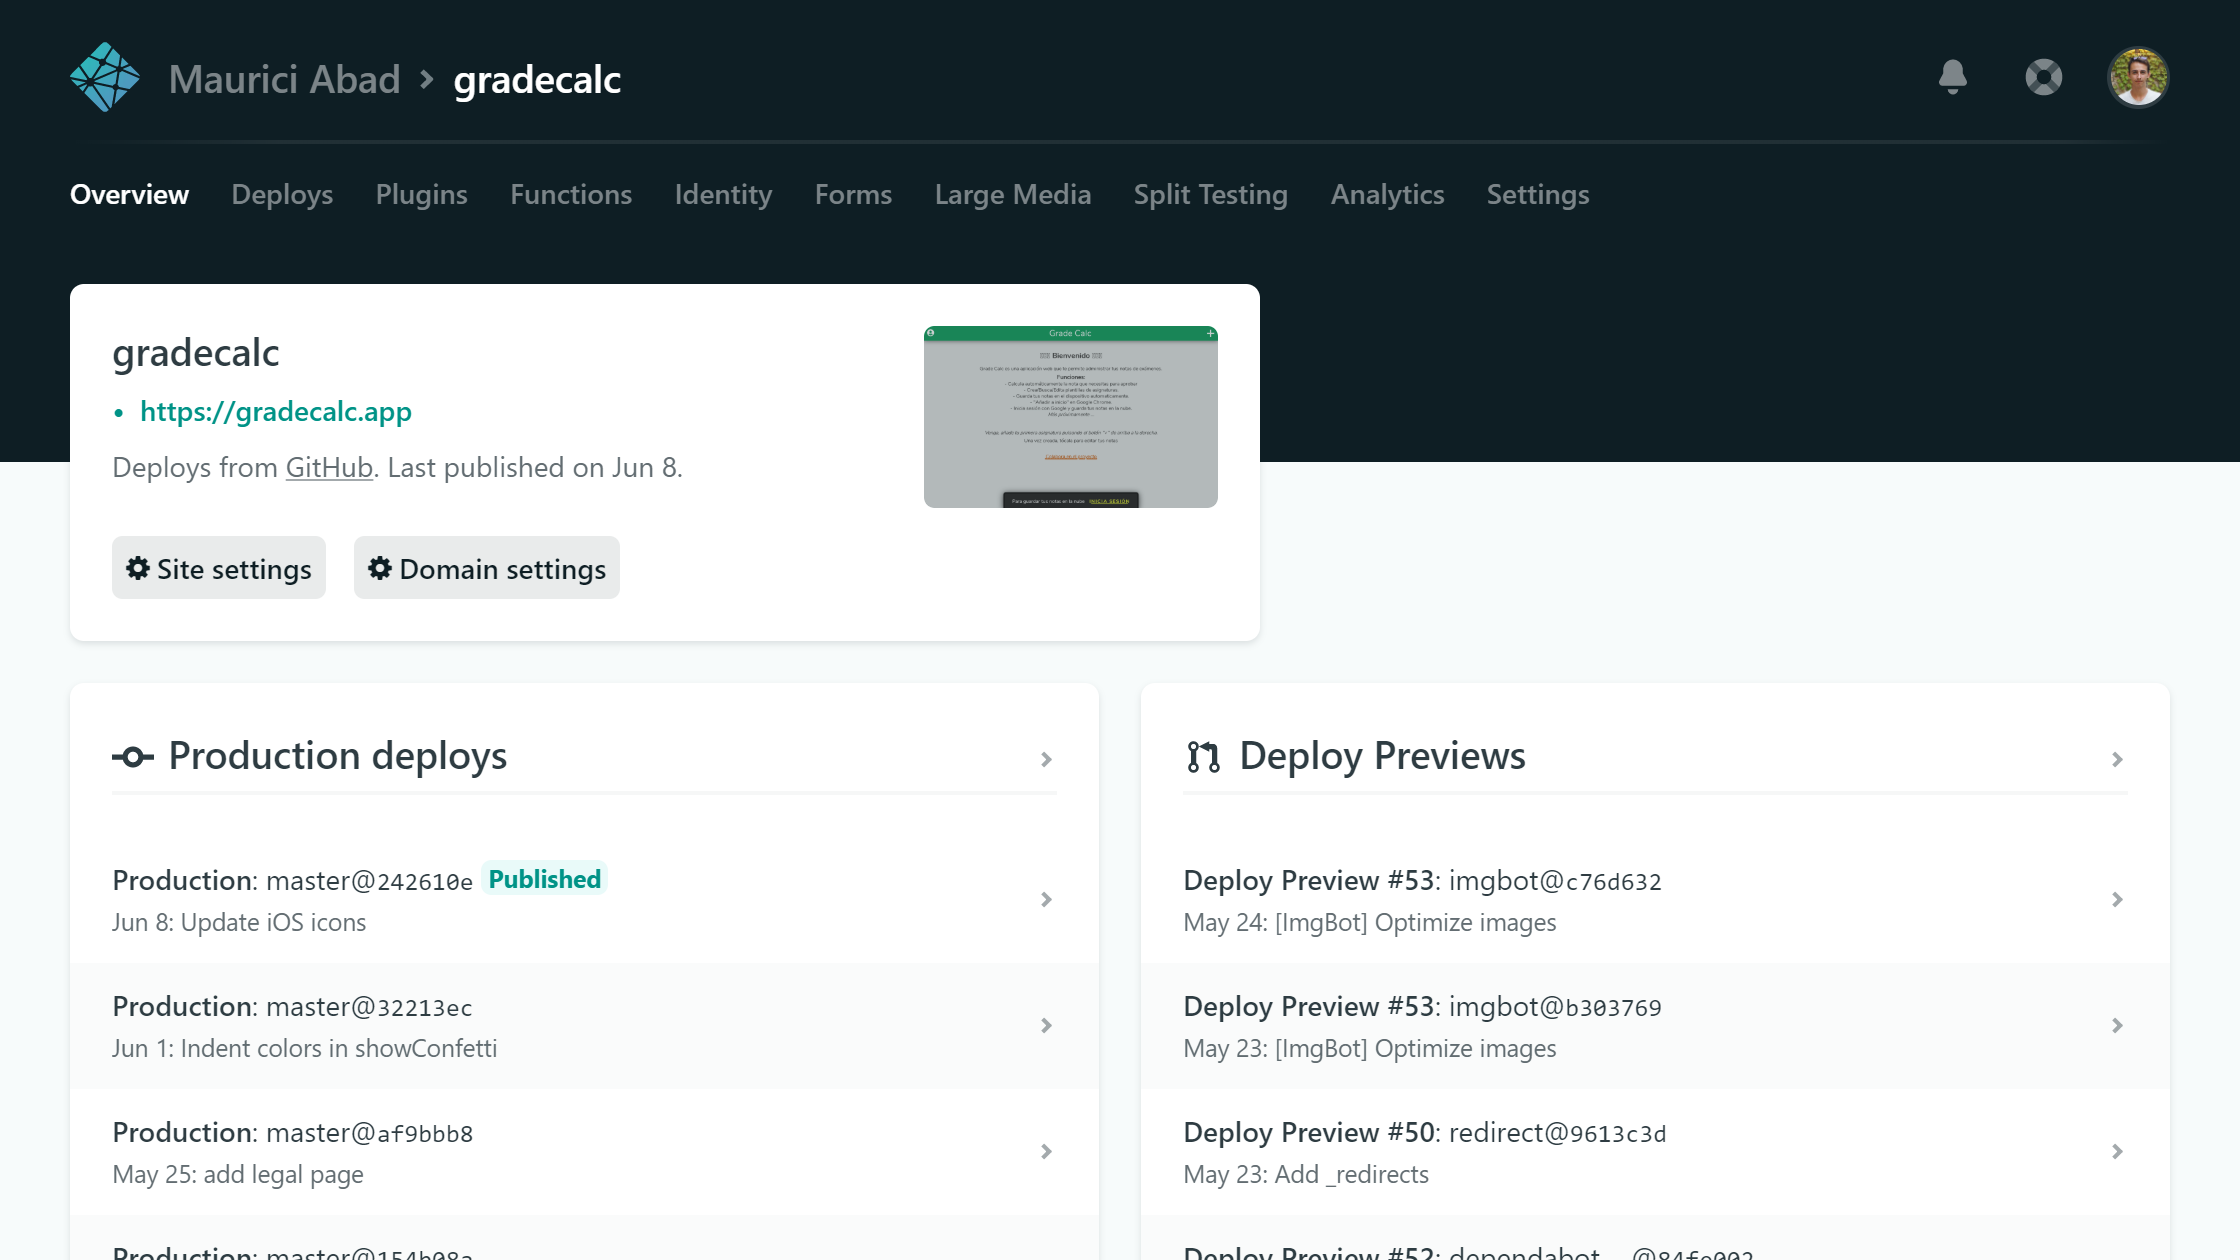
\includegraphics[width=\textwidth]{media/screenshot-netlify-dashboard.png}
%     \caption{Netlify dashboard of GradeCalc}
%     \label{netlify-dashboard}
% \end{figure}
% \vfill